\chapter{Xestión do proxecto}
A xestión do proxecto ten como finalidade definir e alcanzar os obxectivos do mesmo, ó tempo que se optimiza o uso de recursos, tanto humanos como materiais. Na sección III do PMBOK\cite{PMBOK} descríbense amplamente os distintos tipos de procesos que se inclúen dentro da xestión do proxecto, non obstante, para cada proxecto concreto será necesario seleccionar os máis apropiados para cumprir co obxectivo do mesmo.

\section{Alcance do proxecto}
Os procesos de xestión do alcance do proxecto son os encargados de asegurar que o proxecto inclúa o traballo requirido, e só o requirido, para completar o proxecto de forma satisfactoria.

\subsection{Definición do alcance}
O obxectivo deste proxecto é dotar ó Sistema de Información Xeográfica QGIS\footnote{http://www.qgis.org/} da capacidade de consultar fontes de datos SOS e representar os datos obtidos no contorno de mapas proporcionado pola ferramenta, de xeito que podan ser explorados e analizados polo usuario. Para acadar este obxectivo desenvolverase un engadido para o programa QGIS, coas seguintes funcionalidades:

\begin{itemize}
\item Conectarse a un servidor SOS e obter as capacidades do servizo a través da operación GetCapabilities.
\item En base as capacidades do servidor permitir xerar unha petición de observacións, de forma sinxela, sin necesidade de coñecementos técnicos do SOS.
\item Permitir modificar a petición xerada manualmente se o usuario o desexa.
\item Obter as observacións a través da operación GetObservations.
\item Coas observacións descargadas xerar unha capa vectorial que conteña a información xeográfica, temporal e os valores das propiedades observadas.
\item Xerar gráficos en dúas dimensións cos datos da capa.
\item Permitir visualizar a capa co plugin TimeManager de xeito que se podan facer animacións.
\end{itemize}

\subsection{Estrutura de Descomposición do Traballo}
A Estrutura de Descomposición do Traballo (EDT) axuda a dividir o proxecto en paquetes de traballo de forma xerárquica. Dado que se empregará a metodoloxía áxil \emph{Scrum} non é necesario detallar o EDT máis do que xa se fixo no anteproxecto, que se representa na figura \ref{fig:edt}.

\begin{figure}[hbtp]
\centering
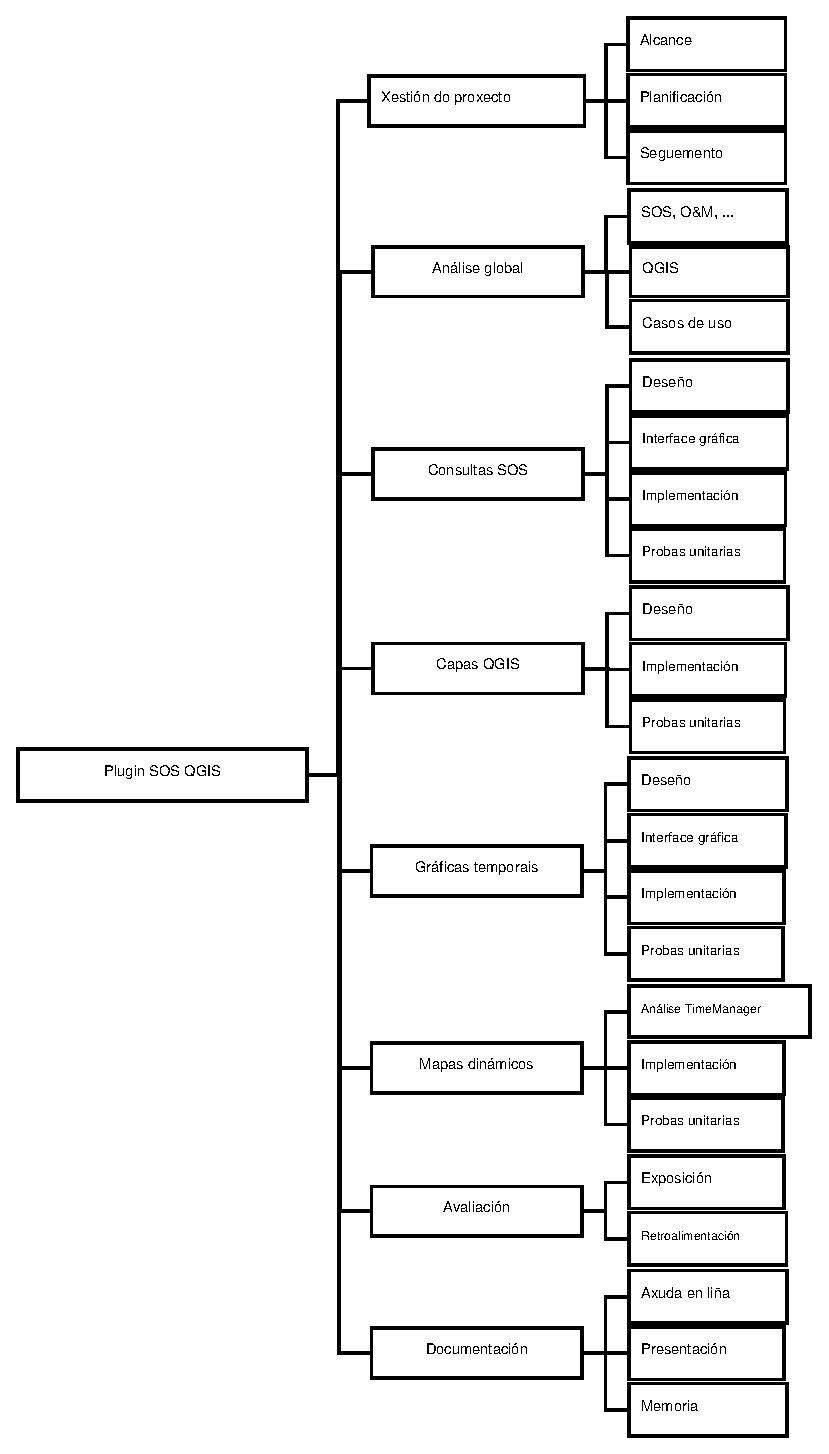
\includegraphics[scale=1]{images/edt.eps}
\caption{Estrutura de Descomposición do Traballo}
\label{fig:edt} 
\end{figure}

\section{Xestión do tempo}
A xestión do tempo do proxecto inclúe os procesos necesarios para lograr a conclusión do proxecto a tempo.

Ó empregar a metodoloxía \emph{Scrum} non se planifica inicialmente a duración de cada tarefa, non obstante si se poden identificar as distintas tarefas a levar a cabo e facer unha estimación da súa duración en base ás horas establecidas para o proxecto e a importancia de dita tarefa para a consecución dos obxectivos do proxecto. Así pois, o diagrama de Gantt da figura \ref{fig:gantt} debe interpretarse como unha estimación das horas a adicar a cada actividade e non como unha organización cronolóxica das actividades a realizar e fitos a acadar.

A continuación enuméranse as fases do EDT \ref{fig:edt} de máis alto nivel describindo a natureza das tarefas que inclúe cada unha delas e que se detallan no diagrama de Gantt \ref{fig:gantt}.

\section{Xestión do custo}
Debido a que este proxecto é un Traballo de Fin de Grao os custos manexados son teóricos e non se considerarán os custos indirectos (electricidade, internet e similares) ou gastos de desprazamento. A xestión de custos faise co único obxectivo de dar unha valoración económica realista do traballo realizado polo que se contemplarán os recursos humanos, os recursos materiais e os recursos software necesarios para a execución do proxecto.

\subsection{Custo de recursos humanos}
O equipo de desenvolvemento para a realización do proxecto consta dunha soa persoa, que realizará as distintas tarefas de análise, programación e documentación do mesmo. Os dous titores do proxecto non se consideran parte do equipo ó nivel de xestión de custos pois a este efecto actúan no rol de clientes.

Consideraremos como salario bruto anual para o recurso 24.000 \euro, que é segundo tecnoempleo.com\cite{InformeSalarios} o salario bruto medio para un analista/programador. Ó salario bruto débense engadir os custos do mesmo para a empresa, que tomando como referencia os datos da Seguridade Social\cite{TabCotizacion} suporía un 29,9\% do mesmo. Para o cálculo do custo por hora considerase a xornada máxima indicada no Convenio Colectivo\cite{BOEConvenio}, que son 1.800 horas de traballo ó ano.

O custo de recursos humanos é por tanto de 17,32 \euro/hora.

\subsection{Custo de recursos materiais}
Para o desenvolvemento do proxecto é necesario un ordenador capaz de executar QGIS. QGIS non especifica formalmente uns requirimentos mínimos e é capaz de funcionar de xeito fluído nun ordenador estándar que se pode adquirir por uns 600 \euro. Considerando unha porcentaxe de amortización anual do 25\%, como indica a Lei 27/2014\cite{Lei27/14}, pódense imputar como custes 12,50 \euro/mes. A estes efectos deben computarse os meses naturais de duración do proxecto.

Os materiais funxibles necesarios para a realización do proxecto e os gastos de impresión e CDs para a presentación do mesmo supoñen un custe de 140 \euro.

\subsection{Custo de recursos software}
Todas as ferramentas software empregadas para a realización deste proxecto son de uso gratuíto.

\subsection{Presuposto}
Na táboa \ref{tab:presuposto} amosase o resumo dos custos do proxecto, que suman un total de \euro.
\begin{table}[H]
\centering
\begin{tabularx}{\textwidth}{Xrrr} \toprule
	Concepto & Cantidade & Custo unitario & Total \\
	\midrule
	Custos de persoal & 420 horas & 17,32 \euro & 7274,40 \euro \\
	Amortización do ordenador & 6 meses & 12,50 \euro & 75,00 \euro \\
	Custos doutros materiais & 1 & 140,00 \euro & 140,00 \euro \\
	\midrule
	\multicolumn{3}{r}{\textbf{Total}} & \textbf{7489,40 \euro} \\
	\bottomrule
\end{tabularx}
\caption{Custos totais}
\label{tab:presuposto}
\end{table}

\section{Xestión de riscos}
A xestión de riscos ten como finalidade aumentar a probabilidade e o impacto de eventos positivos e diminuír a probabilidade e impacto dos eventos adversos para o proxecto. Implica, polo tanto, prever e xestionar os eventos que poden influír na planificación temporal, no esforzo ou no custo do proxecto ou na calidade do produto e tomar as accións necesarias para evitalos ou minimizar o seu impacto. Os catro pasos básicos a seguir para levar a cabo a xestión de riscos son:
\begin{itemize}
\item Identificación
\item Análise e catalogación
\item Planificación da resposta
\item Seguimento e control
\end{itemize}

Para catalogar os riscos en base a súa relevancia empréganse tres medidores: a probabilidade de que ocorra, o impacto que supón sobre o tempo ou esforzo, e o nivel de exposición, que é unha combinación dos valores de probabilidade e impacto. Os distintos valores para estes medidores recóllense na táboa \ref{tab:exposicion}

\begin{table}[H]
\centering
\begin{tabular}{@{}ccccc@{}}
\cmidrule(l){3-5}
\multicolumn{2}{c}{\multirow{2}{*}{}}                                                                       & \multicolumn{3}{c}{Probabilidade}                                                                                                                                                                                    \\ \cmidrule(l){3-5} 
\multicolumn{2}{c}{}                                                                                        & \begin{tabular}[c]{@{}c@{}}Case seguro\\ $\geq$80\%\end{tabular} & \begin{tabular}[c]{@{}c@{}}Moi probable\\ \textless80\% e \textgreater30\%\end{tabular} & \begin{tabular}[c]{@{}c@{}}Pouco probable\\ $\leq$30\%\end{tabular} \\ \midrule
\multirow{6}{*}{\rotatebox{90}{Impacto}} & \begin{tabular}[c]{@{}c@{}}Alto\\ $\geq$20\%\end{tabular}                & Alto                                                             & Alto                                                                             & Medio                                                          \\
                         & \begin{tabular}[c]{@{}c@{}}Medio\\ \textless20\% e \textgreater10\%\end{tabular} & Alto                                                             & Medio                                                                            & Baixo                                                          \\
                         & \begin{tabular}[c]{@{}c@{}}Baixo\\ $\leq$10\%\end{tabular}                   & Medio                                                            & Baixo                                                                            & Baixo                                                          \\ \bottomrule
\end{tabular}
\caption{Nivel de exposición dun risco en base a Probabilidade e Impacto}
\label{tab:exposicion}
\end{table}

\subsection{Especificación de riscos}
Co obxectivo de non engadir complexidade ó seguimento do proxecto so se planifican os riscos adversos con un nivel de exposición alto, é dicir, os riscos que é bastante probable que ocorran e que teñen un impacto negativo considerable sobre o desenvolvemento do proxecto. Para desenvolver respostas efectivas ós riscos é de moita utilidade agrupalos por causas comúns, neste caso clasificándoo en base á fonte do risco.

\subsubsection{Riscos técnicos}
\risktable	{R.TEC.01}{Complexidade do estándar SOS} %Id, Nome
			 %Descrición
		  	{O nivel de madurez e uso do estándar SOS fai que sexa un estándar extremadamente amplo e con un alto grao de liberdade. Non existe ningunha implementación que cubra o estándar na súa totalidade.}
			{Moi probable} %Probabilidade
			{Alto} %Impacto
			{Alto} %Nivel de exposición
			%Resposta
			{Só se comprometerá como imprescindible soportar as operacións básicas para obter os datos de observacións provistos pola implementación SOS realizada polo CiTIUS.}

\risktable	{R.TEC.02}{Escaseza de servidores SOS} %Id, Nome
			 %Descrición
		  	{Existen moi poucos servidores que implementen SOS abertos ó público cos que poder validar a implementación realizada.}
			{Case seguro} %Probabilidade
			{Medio} %Impacto
			{Alto} %Nivel de exposición
			%Resposta
			{Instalar en local un servidor SOS para poder probar a aplicación, e solicitar acceso ós xestionados polo CiTIUS.}
			
\subsubsection{Riscos externos}
\risktable	{R.EXT.01}{Soporte de SOS en QGIS} %Id, Nome
			 %Descrición
		  	{Implementación nativa dentro do QGIS do soporte para SOS ou a publicación de algún plugin que implemente dito soporte.}
			{Moi probable} %Probabilidade
			{Alto} %Impacto
			{Alto} %Nivel de exposición
			%Resposta
			{Reorientar o proxecto para centralo en dotar o QGIS de ferramentas específicas para interacción cos datos de sensores, sempre e cando a solución SOS implantada de soporte a implementación realizada polo CiTIUS.}

\subsubsection{Riscos de persoal}
\risktable	{R.PER.01}{Descoñecemento da ferramenta QGIS} %Id, Nome
			 %Descrición
		  	{O equipo de desenvolvemento non ten experiencia no manexo da ferramenta QGIS nin outras ferramentas de información xeográfica.}
			{Case seguro} %Probabilidade
			{Medio} %Impacto
			{Alto} %Nivel de exposición
			%Resposta
			{No plan de traballo do proxecto inclúese capacitación na ferramenta QGIS así como nos conceptos básicos sobre sistemas de información xeográfica.}

\risktable	{R.PER.02}{Descoñecemento da linguaxe Python} %Id, Nome
			 %Descrición
		  	{O equipo de desenvolvemento non ten experiencia na linguaxe de programación Python.}
			{Case seguro} %Probabilidade
			{Alto} %Impacto
			{Alto} %Nivel de exposición
			%Resposta
			{No plan de traballo do proxecto inclúese capacitación na linguaxe de programación Python PyQt4.}
			
\risktable	{R.PER.03}{Situación persoal dos membros do equipo} %Id, Nome
			 %Descrición
		  	{Cambios na situación persoal ou laboral nos membros do equipo que impidan levar a cabo a dedicación estimada.}
			{Case seguro} %Probabilidade
			{Alto} %Impacto
			{Alto} %Nivel de exposición
			%Resposta
			{Volver a planificar os prazos de execución do proxecto.}
			
\subsubsection{Riscos na xestión do proxecto}
\risktable	{R.XES.01}{Error na estimación temporal} %Id, Nome
			 %Descrición
		  	{A estimación temporal inicial para a execución das tarefas é pouco precisa a causa da inexperiencia en proxectos similares.}
			{Case seguro} %Probabilidade
			{Medio} %Impacto
			{Alto} %Nivel de exposición
			%Resposta
			{A estimación inicial realizase de forma pesimista. A metodoloxía \emph{Scrum} minimiza o impacto ó permitir a refinación de requisitos e estimacións o longo do proxecto.}

\section{Xestión da configuración}
A xestión da configuración \cite{GPGC} ten como propósito establecer e manter a integridade dos elementos de traballo. No proxecto que nos ocupa os elementos de traballo a xestionar son o código fonte do \emph{plugin}, o código fonte da documentación, e os distintos entregables xerados.

\subsection{Control do código fonte}
Dentro do código fonte a xestionar inclúese tanto o código do aplicación, imaxes, documentos de axuda e demais que si inclúen no \emph{plugin} empaquetado, como o código fonte para xerar a documentación.

En ambos casos o procedemento de xestión da configuración se fai a través do sistema de xestión de versións \emph{Git}. Mantéñense en local dous repositorios diferentes, un para aplicación e outro para documentación, cada un coa súa réplica remota correspondente aloxada en \emph{GitHub}\footnote{https://github.com/}. As carpetas dos repositorios locais replícanse en Dropbox\footnote{https://www.dropbox.com/} co obxectivo de ter unha copia redundante na nube e acceso desde distintos ordenadores en todo momento.

O método de traballo consiste en realizar un \emph{Commit} local cada vez que se remata unha tarefa e realizar un \emph{Push} ó servidor remoto cada vez que se remata unha versión susceptible de ser publicada. Deste xeito no repositorio público sempre hai unha versión estable do produto.

\subsection{Control dos entregables}
Os distintos obxectos entregables xerados o longo do proxecto, dende o anteproxecto ata a presentación do mesmo son arquivados tanto en local como na carpeta de Dropbox. Non se realiza máis control de versións sobre os produtos entregables que o propio control realizado por Dropbox. Esta ferramenta permite o acceso ás distintas versións gardadas de calquera tipo de ficheiro.

O servizo Dropbox tamén permite a creación de carpetas públicas. Esta funcionalidade permítenos crear un repositorio público para QGIS no que aloxar o \emph{plugin} empaquetado de xeito que sexa moi sinxelo de instalar.